\documentclass[a4paper, onecolumn, 12pt]{article}
\usepackage[left=32mm,right=32mm,top=35mm,columnsep=15pt]{geometry} 

% basic packages
\usepackage[english]{babel} %language
\usepackage[utf8]{inputenc} %input encoding
\usepackage{float} %position of floating objects
\usepackage{bookmark} %hyperlinks in pdf
\usepackage{subcaption}
\usepackage[T1]{fontenc}
\usepackage{lipsum} %placeholder text

% math packages
\usepackage{amsthm} %theorems
\usepackage{amsmath} %math
\usepackage{mathtools} %still math

% code packages
\usepackage{listings} %code
\usepackage{xcolor} %syntax highlighting
\usepackage{algorithm}
\usepackage{algpseudocode}
\usepackage{fancyvrb}

% todonotes package
\usepackage{xkeyval}
\usepackage{tikz}
\usepackage{calc}
\setlength {\marginparwidth }{2cm}
\usepackage{todonotes} % Load the todonotes package

% custom commands
\newcommand\tab[1][.3cm]{\hspace*{#1}}
\newcommand\tabeq[1][.5cm]{\hspace*{#1}}

% \usepackage{physics}
% \usepackage{adjustbox}
% \usepackage{placeins}
% \usepackage{csquotes}
% \usepackage[normalem]{ulem}
% \useunder{\uline}{\ul}{}

\title{Long-Horizon Vehicle Motion Planning and Control Through Serially Cascaded Model Complexity: Implementation and Experimentation}
\author{Flavio Maiorana \and Flavio Volpi \and Andrea Ferrari}
\date{\today}

\begin{document}

\listoftodos

\maketitle
\begin{abstract}
    Dynamical models can be too computationally expensive for real-time
    purposes, especially when they have to be accurate. The proposal of
    \cite{paper} is to devise an MPC algorithm where the horizon is split in two
    parts, with the first driven by an accurate model and the second by a
    simpler one. We propose the implementation and experimentation of a motion
    planning and control framework for autonomous vehicles based on nonlinear
    model-predictive control, inspired by \cite{paper}. Our main contribution is
    the development of the algorithm and a graphical simulator to test it. We've
    also added some additional benchmarks that involve the presence of obstacles
    on the track. The code is publicly available at
    \href{https://github.com/neverorfrog/vehicle-control}{this GitHub
    repository}.
\end{abstract}

\newpage
\tableofcontents

\newpage
\section{Introduction and related works}

In recent years autonomous driving has emerged as one of the most prominent topics in the robotics and artificial intelligence research fields, while also gathering a lot of attention from the general public. It has the potential to reshape the way we move around a city completely, and can lead to a significant reduction of deaths related to road accidents.

The main challenges of autonomous driving are ensuring the ability to accurately perceive the environment surrounding the vehicle, and then solve complex decision-making problems based on the received data. Nevertheless,  at the heart of autonomous driving lies the challenge of motion planning, which is the process of determining the optimal path and speed, while respecting various constraints, such as safety, speed and many others.

To approach this challenge, one popular approach is to employ Model Predictive Control (MPC), which is a control technique that, in closed-loop, computes the control inputs by means of an optimization algorithm,
which uses a \textbf{model} of the system and measurements to \textbf{predict}
future states and act accordingly by choosing the "best" control action. 

\begin{equation}
\begin{aligned}
    \min_{u_0,...,u_{N-1}}{J(x,u)} \\
    \text{ subject to }
        \quad x_{k+1} = f(x_k,u_k) \\
        \quad x_0 = x(t) \\
        \quad u_{min} \leq u_k \leq u_{max}
\end{aligned}
\end{equation}

We call $J(x)$ the \textbf{cost function} and $f(x,u)$ the \textbf{model}. The
critical part of MPC lies in the two last rows. The second-last expresses the
fact that, for every planning horizon, the current state is the initial state:
this is a subtle but important difference with respect to, for example,
trajectory optimization. The last row entails an equally important concept which
pertains specifically MPC, namely constraints. In the end, the sequence of
control actions is generated such that the cost function is minimized over the
\textbf{prediction horizon} by solving a constrained optimization problem that
depends on the evolution of the model over the horizon itself. Then, the
controller applies just the first action: in this way the system has advanced
one step, a new optimization problem with a new initial state is produced, and
the process goes on. The advantages of MPC are many: it is a multivaribale
controller, so it can control outputs by handling simultaneously all the
interactions between system variables; as said, it can handle constraints, so it
allows to avoid possible undesired states; it predicts the future states,
allowing to incorporate their information in the actual control. It is
particulary useful for a real-time control that adapts to \textbf{changes in the
environment}.\\
When dealing with nonlinear dynamics, a nonlinear MPC (or NMPC) can be used to
capture more accurately the nonlinear behavior of a system. This entails a more
robust manipulation capability of both nonlinearities and uncertainties in the
system. However, one of its major problems is the computational power it can
require, especially when dealing with highly nonlinear systems. This entails the
need of a high-performance hardware to solve the optimization problem in an
acceptable time, but sometimes this is not enough. Especially in a real
environment, where the timeliness is fundamental to take a decision,
computational efficiency is of utmost importance.

This is especially true for the task of autonomous driving, where there is the need for a long planning horizon, due to the high speeds reached by the vehicle, which require it to start braking well in advance for upcoming turns in the road, and the need for a fast control loop in order to stabilize the vehicle and avoid any unexpected obstacle.

Due to the duality of the requirements, a popular approach has been to use different control loops to address different tasks. In \cite{Gros2007} for example, to control a quadcopter with similar requirements to our case, two loops with different time scales were used: a slow trajectory generation loop and a faster loop for controlling said quadcopter through linear feedback. 

Another approach has been to use two models of different complexity, to deal with different tasks. In \cite{Gao2010} a point-mass model is used for high-level path planning, while a more complex four-wheel model is used for low-level path following.

The main limitation of this approach is that the trajectory generated by the high-level path planner might be feasible for the simple point-mass model but impossible to track by the low-level controller, that has to control a more complex model, with more constraints and limitations.\\

\cite{paper} follows the intuition of using models of different complexity, and improves on it by employing a so-called \textbf{cascaded model}, composed by a
detailed model of the car for the near term, and a simpler model used for
planning in the long term. 
This leads to the developement a novel, more computationally
cost-effective approach for a real-time NMPC for a autonomous driving, which
was tested in a race environment, where the objective was to complete a lap in
the minimum possible time, considering the actual capabilities of the vehicle. 

In this work we tried to replicate the architecture of the paper from scratch,
testing the code in a very simple simulated race environment. Our purpose is to
show that, as claimed by \cite{paper}, the average computation time for the
cascaded model is lower, achieving also better results in terms of lap time.


\subsection*{Related Work}

\todo[inline]{Fare related work}

\begin{itemize}
    \item Learning-based approach for vehicle control in \cite{rosolia}
    \item Linearization approach in \cite{bemporad}
\end{itemize}


\subsection*{Outline}

In the next section we will address the modeling part of the algorithm in a
rather formal way. Then, we will formalize the NLP structure and put everything
together to define the complete MPC problem. Right after, we will discuss about
the actual implementation. In the end, we will discuss some experiments and the
results.


\newpage
\section{Models}

Models must be well-defined to be used in NMPC. It is important to note that, as
said in \cite{paper}, the cascaded model together with the NLP formulation has
the precise goal to solve the problem of pushing a car to its physical
boundaries, like in race, while maintaining real-time performance. In this
section we will describe the main concepts behind the modeling part of the NMPC
algorithm. 

\subsection{Serially cascaded dynamical model}
Broadly speaking, while a single control loop system is a simple structure that
consists in just one primary loop that regulates directly the system, the
cascade control makes use of multiple control loops nested within each other.
The requirements for an effective cascade control are that the inner loops
variables must be faster-responding than the outer ones, and the major
disturbances enter in the inner loops. Considering the simplest cascade control
structure,\\
... (aggiungi schema/equazioni generiche del cascade semplice)

According to the control objectives, a cascade control scheme can include also 
more than one model in its control loops, such that each model capture different
relevant dynamics meeting different control tasks. In this way there is not the 
need to use a high-fidelity model for every objective, because some of them can 
be achieved considering simpler dynamic models. Furthermore, in optimal control
the usage of detailed models for long horizon can bring to an explosion of the 
complexity of the problem; instead, using more detailed models for near terms 
to have a high-fidelity of the real robot, and easier models for planning purpose
in long terms, allows to achieve good performances with computational limits.

When dealing with more than one dynamic model with different dynamic speeds,
the main advantage of a cascade control scheme is the higher performace with respect
to a simple single control loop, thanks to the possibility to control disturbances
in the inner loop before they affect the outer one. The main problem this architecture
can face is in the interaction between the control loops, where the reference signals 
generated by a control loop are not achievable by the others. This happens especially
when we are dealing with models with different complexity levels.

To deal with the disadvantages of the cascade control design, but leveraging on
its strengths, the idea of \cite{paper} in the scenario of an autonomous car is
to build a serial architecture which contains two dynamic models, belonging to
the same single control loop and the same prediction horizon. The first one is a
single-track vehicle model, which reflects comprehensively the complex dynamic
of the car (we will see in the next section the details) and provides all the
tools to accurately treat the first prediction steps. The farthest window of the
horizon is treated with a planar point-mass model, useful for long-term
trajectory planning with low computational resources. Thus the benefits of the
cascade model for the trajectory task are preserved; moreover the existance of a
single control loop ensure the feasibility of the reference targets that are
exchanged between the two models. A very important aspect to pay attention to
lies in the linkage of the plant models, namely propagating correctly the final
state of the first model to the initial state of the second model, and
mantaining consistency in constraints and cost functions across interconnected
models. 


\subsubsection{Single-track dynamic model}
The car can be represented as a dynamic bicycle model, where the two pairs of
front and rear wheels can be merged into a single wheel, one front wheel and one
rear wheel.\\
For the intrinsic properties, the vehicle is assumed to have a mass $\mathbf{m}$
and a yaw moment of inertia $\mathbf{I_{zz}}$; the wheelbase has length
$\mathbf{L}$, divided into $\mathbf{a}$ and $\mathbf{b}$, where they are
respectively the distances between the Center of Gravity and the front and rear
axle; the CG is at a distance $\mathbf{h_{cg}}$ from the ground; the front steer
angle is $\mathbf{\delta}$.\\
Since the model is of second-order, the state is composed of a velocity
component and a position/orientation one. The first one consists of the
longitudinal speed $\mathbf{U_x}$, the lateral speed $\mathbf{U_y}$, and the yaw
rate $\mathbf{r}$ of the CG. Meanwhile, the pose component is expressed in
relative coordinates withe respect to the road descriptor, namely by the
curvilinear coordinate $\mathbf{s}$, the lateral distance $\mathbf{e}$, and the
orientation of the chassis $\mathbf{\Delta \varPsi}$ with respect to the road
descriptor path. The curvature of the path, which is necessary to compute the
curvilinear coordinate and the orientation is called $\mathbf{\kappa}$. Thus, we
can at every time instant identify a unique pose of the vehicle by the tuple
$s,e,\Delta \varPsi$, as already said in section \ref*{subsec:track}.\\
The inputs of the system are the steering angle rate $\dot{\delta}$ and the
total longitudinal force $F_x$. This one can be divided in the longitudinal
force applied on the axle of the front tire $F_{x_f}$ and the longitudinal force
applied on the axle of the rear tire $F_{x_r}$, according to a distribution
function $\tilde{\chi}$:
\begin{subequations}
    \begin{eqnarray}
        \tilde{\chi_f} &=& \frac{d_f - b_f}{2}\tanh(2(F_x+0.5))+\frac{d_f+b_f}{2} \\
        \tilde{\chi_r} &=& \frac{b_r-d_r}{2}\tanh(-2(F_x+0.5))+\frac{d_r+b_r}{2}
    \end{eqnarray}
\end{subequations}
where $d_f$ and $d_r$ represent the drive force distribution, and $b_f$ and $b_r$ represent the 
brake force distribution. So the single components of the longitudinal force are:
\begin{subequations}
    \begin{eqnarray}
        \tilde{F}_{x_f} &=& \tilde{\chi}_f(F_x) \cdot F_x \\
        \tilde{F}_{x_r} &=& \tilde{\chi}_r(F_x) \cdot F_x
    \end{eqnarray}
\end{subequations}
This implementation might seem rather complex, compared to simply expressing the front and rear force distribution as
\begin{subequations}
    \begin{eqnarray}
        \tilde{F}_{x_f} = \tilde{\chi}_f \cdot F_x \\
        \tilde{F}_{x_r} = \tilde{\chi}_r \cdot F_x
    \end{eqnarray}
\end{subequations}
where $\tilde{\chi}_f$ and $\tilde{\chi}_r$ are scalars that sum to 1, however, these equations will be used for numerical 
optimization, and should therefore be twice differentiable, and we therefore have to use the workaround equations presented above. \\
For the tire model, given the maximum instantaneous normal load of the tire $F_z$, the maximum possible
lateral tire force that can be obtained applying the input force $\tilde{F}_x$ is:
\begin{equation}
    \tilde{F}_y^{max} = \sqrt[]{(\mu F_z)^2 - (0.99\cdot \tilde{F}_x)^2}
\end{equation}
where $\mu$ is the tire-road friction coefficient and the 99\%  of the longitudinal force is due to solve 
some numerical issues in the optimization problem. \\
The normal loads for the two tires are affected also by the slope $\theta$ of the road, and by the banking $\phi$, in the following way:
\begin{subequations}
    \begin{eqnarray}
        \label{normal}
        F_{z_f} = \frac{b}{L}m(g\cdot \cos(\theta)\cos(\varphi)+A_{V^2}U_x^2)-\frac{h_{cg}}{L}F_x \\
        F_{z_r} = \frac{a}{L}m(g\cdot \cos(\theta)\cos(\varphi)+A_{V^2}U_x^2)+\frac{h_{cg}}{L}F_x
    \end{eqnarray}
\end{subequations}
where the effect of vertical curvature on speed are expressed through:
\begin{equation}
    A_{V^2} = -\frac{\partial \theta}{\partial s}\cos(\varphi)-\kappa\cdot \sin(\varphi)\cos(\theta) 
\end{equation}
The slip angles of the front ($\alpha_f$) and rear ($\alpha_r$) wheels are respectively given by:
\begin{subequations}
    \begin{eqnarray}
        \alpha_f &=& \arctan \left(\frac{U_y+ar}{U_x}\right)-\delta \\
        \alpha_r &=& \arctan \left(\frac{U_y-br}{U_x}\right)
    \end{eqnarray}
\end{subequations}
A full sliding occurs at an angle denoted as $\alpha^{\text{mod}}$, which is calculated as:
\begin{equation}
    \alpha^{\text{mod}} = \arctan\left(\frac{3\cdot F_y^{\text{max}}\cdot\zeta}{C_{\alpha}}\right)
\end{equation}
Here, $\zeta$ is a factor introduced to ensure the tire model's strict monotonicity.\\
Thus, considering $\alpha = \left(\alpha_f \tab \alpha_r\right)^T$, the tire model can
be expressed as:
\begin{equation}
    F_y = 
    \left\{
	\begin{array}{ll}
		-C_\alpha \tan(\alpha)+&\\
        \tabeq\frac{C_\alpha^2}{3\tilde{F}_y^{max}}|\tan(\alpha)|\tan(\alpha) - &\\
        \tabeq\frac{C_\alpha^3}{27(\tilde{F}_{y}^{max})^2}\tan^3(\alpha) 
        & \mbox{if } |\alpha| \leq \alpha^{mod} \\
		-C_{\alpha}(1-2\zeta+\zeta^2)\tan(\alpha)-&\\
        \tabeq \tilde{F}_y^{max}(3\zeta^2-2\zeta^3){sgn(\alpha)}
        & \mbox{otherwise }
	\end{array}
    \right.
\end{equation}
\\
Regarding the drag forces, these are included all in the same variable $F_d$:
\begin{equation}
    \label{drag_force}
    F_d = F_{rr}+C_DU_x^2-mg\sin(\theta)
\end{equation}
where $F_{rr}$ represents the rolling resistance, $C_D$ is the coefficient of aerodynamic
drag. \\
Instead, the lateral force $F_b$ applied on the CG models the effect of the road bank angle $\varphi$:
\begin{equation}
    \label{lateral_force}
    F_b = -mg\cos(\theta)\sin(\varphi)
\end{equation}
\\
\\
All these informations are used to describe the motion of the single-track model:
\begin{subequations}
    \begin{eqnarray} 
        \dot{U}_x &=& \frac{\tilde{F}_{x_f}\cos(\delta)-\tilde{F}_{y_f}\sin(\delta)+\tilde{F}_{x_r}-F_d}{m}+rU_y\\
        \dot{U_y} &=& \frac{\tilde{F}_{y_f}\cos(\delta)+\tilde{F}_{x_f}\sin(\delta)+\tilde{F}_{y_r}+F_b}{m}-rU_x\\ 
        \dot{r} &=& \frac{a(\tilde{F}_{y_f}\cos(\delta)+\tilde{F}_{x_f}\sin(\delta))-b\tilde{F}_{y_r}}{I_{zz}}\\
        \dot{s} &=& \frac{U_x\cos(\Delta \varPsi) -U_y\sin(\Delta \varPsi)}{1-\kappa e}\\
        \dot{e} &=& U_x\sin(\Delta \varPsi)+U_y \cos(\Delta \varPsi)\\
        \Delta \dot{\varPsi} &=& r-\kappa \dot{s}
    \end{eqnarray}
\end{subequations}

\subsubsection{Point-Mass model}
The Point-Mass model is a simpler version of the Single-Track model, where the car is approximated with a point object
in the Center of Gravity of the vehicle. Being a one-dimensional object, the point has just one total horizontal velocity state $\bar{V}$, 
and three position states relative to the road descriptor path: the distance $\bar{s}$ along it, the lateral distance $\bar{e}$ from it, and finally the
difference in orientation $\bar{\phi}$ between the velocity vector and the tangent to the road descriptor path.

Substituting ${U}_x$ with $\bar{V}$, we can use some of the equations introduced in the single-track model also for the point-mass model,
in particular for the drag force ${F}_d$ (eq. \ref{drag_force}), for ${F}_b$ (eq. \ref{lateral_force}) and for the normal loads ${F}_{z_f}$ and ${F}_{z_r}$ (eq. \ref{normal}).
Following the basic intuition of having to simplify the model, the tire forces are not modeled.

The inputs to this model are the longitudinal force $\bar{F}_x$ and the lateral force $\bar{F}_y$, that are limited by friction limits
according to the following rules:
\begin{subequations}
    \begin{eqnarray} 
        \left(\frac{b}{L}\bar{F}_y\right)^2 + \left(\tilde{\chi_f}\bar{F}_x\right)^2 \leq \left(\mu_f F_{z_f}\right)^2 \\
        \left(\frac{a}{L}\bar{F}_y\right)^2 + \left(\tilde{\chi_r}\bar{F}_x\right)^2 \leq \left(\mu_r F_{z_r}\right)^2
    \end{eqnarray}
\end{subequations}
Thus the equations that describe the motion of the point-mass model are the following:
\begin{subequations}
    \begin{eqnarray}
        \dot{\bar{V}} &=& \frac{\bar{F}_{x}-\bar{F}_{d}}{m}\\
        \dot{\bar{s}} &=& \frac{\bar{V}\cos(\bar{\phi})}{1-\kappa \bar{e}}\\
        \dot{\bar{e}} &=& \bar{V}\sin(\bar{\phi})\\
        \dot{\bar{\phi}} &=& \frac{{\bar{F}}_y + {\bar{F}}_b}{m\bar{V}} - k\dot{\bar{s}}
    \end{eqnarray}
\end{subequations}

Note that the yaw dynamics are omitted, and therefore this model cannot be used for yaw stabilization

\subsubsection{Propagating the state from single-track to point-mass}
Here we define the mapping from the single-track to the point-mass states. 
It is very important that this mapping is correct, to guarantee that the transition
from one model to the other is compliant to the reality.\\
The mapping, called $spatialTransition_{trans}(x_k)$, is the following:
\begin{subequations}
    \begin{eqnarray}
        \bar{V} &=& \sqrt{U_{x}^{2}-U_{y}^{2}}\\
        \bar{s} &=& s\\
        \bar{e} &=& e\\
        \bar{\phi} &=& arctan\left(\frac{{U}_y}{{U}_x}\right) + \Delta\psi
    \end{eqnarray}
\end{subequations}

\subsection{Spatial dynamics} \label{spatial}
Since the dynamical models need to be used in a digital fashion, it has to be
discretized. The discretization of the models can be done with respect to time
or with respect to space, according to own purposes, with the respective pros
and cons.
\begin{description}
    \item[Discretizing in time] consists in dividing the time over the horizon in
    small well-defined time intervals $dt$, and leaving the spatial curvilinear
    coordinate $s$ as an optimization variable in the NLP. This approach implies
    that we know beforehand the temporal window for the horizon. Since this is
    the most straightforward wa to discretize, it is also more intuitive.
    Nevertheless, there are some problems attached to it, especially in a car
    racing scenario. Since the curvilinear abscissa acts as a variable, it
    cannot be keep fixed inside of a single time interval, which means that the
    path geometry will be obtained by some interpolation function to be
    evaluated during the planning horizon. This can cause some issues,
    computation-wise.
    \item[Discretizing in space] means to establish the spatial
    discretization steps $ds$ that compose the total space travelled by the
    vehicle in the horizon window. In this way the time $t$ can be left as an
    optimization variable. In contrast, this method does not allow to the car to
    stop, but this is not a problem for our purposes. Instead, a good advantage
    of the spatial discretization is that during each \textbf{space interval},
    the path geometry is known and constant, and thus can be computed apriori,
    before even starting the planning horizon. Moreover, space discretization
    allows to easily add elements to the track which are always know apriori,
    like static obstacles, without creating too much trouble.
\end{description}
For the reasons stated above, since we are a racing scenario in which time
minimization is of paramount importance, and the track geometry is known
apriori, the spatial discretization method is the more adequate for the MPC
planning horizon. This means that outside the horizon, the dynamical model will
evolve as usual, following a time-discretized differential equation, while
inside the MPC the evolution is space-disretized. Thus, denoting as $p$ a state
variable of any model, we define its derivative with respect to the curvilinear
coordinate $s$ as
\begin{equation}
    p' = \frac{d p}{d s} = \frac{dp}{dt} \frac{dt}{ds} = \dot{p} \frac{dt}{ds} = \dot{p} \frac{1}{\dot{s}}
\end{equation}  
that we will compute through the chain rule.
According to this notation, we can define the spatial dynamics for the single-track model as such:
\begin{subequations}
    \begin{eqnarray}
        U'_x &=& \left(\frac{\tilde{F}_{x_f}\cos(\delta)-\tilde{F}_{y_f}\sin(\delta)+\tilde{F}_{x_r}-F_d}{m}+rU_y\right) \frac{1}{\dot{s}}\\
        U'_y &=& \left(\frac{\tilde{F}_{y_f}\cos(\delta)+\tilde{F}_{x_f}\sin(\delta)+\tilde{F}_{y_r}+F_b}{m}-rU_x\right) \frac{1}{\dot{s}}\\
        r' &=& \left(\frac{a(\tilde{F}_{y_f}\cos(\delta)+\tilde{F}_{x_f}\sin(\delta))-b\tilde{F}_{y_r}}{I_{zz}}\right) \frac{1}{\dot{s}}\\
        e' &=& \left(U_x\sin(\Delta \varPsi)+U_y \cos(\Delta \varPsi)\right) \frac{1}{\dot{s}}\\
        \Delta \varPsi' &=& \left(r-\kappa \dot{s}\right) \frac{1}{\dot{s}}\\
        \delta ' &=& \frac{\dot{\delta}}{\dot{s}}\\
        t' &=& \frac{1}{\dot{s}}
    \end{eqnarray}
\end{subequations}
and for the point-mass model:
\begin{subequations}
    \begin{eqnarray}
        {\bar{V}}' &=& \left(\frac{\bar{F}_{x}-\bar{F}_{d}}{m}\right) \frac{1}{\dot{\bar{s}}}\\
        {\bar{e}}' &=& \left(\bar{V}\sin(\bar{\phi})\right)\frac{1}{\dot{\bar{s}}}\\
        {\bar{\phi}}' &=& \left(\frac{{\bar{F}}_y + {\bar{F}}_b}{m\bar{V}} - k\dot{\bar{s}}\right)\frac{1}{\dot{\bar{s}}}\\
        \bar{t}' &=& \frac{1}{\dot{\bar{s}}}
    \end{eqnarray}
\end{subequations}
We will denote in a concise way the spatial transitions from a state to the next one as
$spatialTransition_{st}(x_k, u_k)$ for the single-track, and $spatialTransition_{pm}(x_k, u_k)$ 
for the point-mass model, where $x_k$ is the state at time step $k$ and $u_k$ is the control
applied at time step $k$. \\
It is important to add that this model is subject to a singularity when $U_x=0$
or $\bar V=0$, caused by the spatial step size becoming infinitely large. This
can be addressed by using a kinematic model at low speeds. We will address this
point in the experiments section. 


\newpage
\section{NLP Structure}
The NLP (non-linear program) has three main components:
\begin{itemize}
    \item Decision variables (state and action)
    \item Cost function
    \item Constraints
\end{itemize}

\subsection{Cost function}\label{cost_section}

Our objective is to minimize time (which, we remind, has to be integrated in the
spatial step and thus is not know before starting the prediction horizon) at
each "space instant" along the finite planning horizon, while also respecting
the road boundaries and while keeping the car in a safe configuration. To
achieve this, a series of terms regarding both single-track and point-mass
models are summed together in the cost function. In general, we will have $N$
steps for the singletrack model and $M$ steps for the pointmass model.
\begin{enumerate}
    \item \textbf{Final time}: the time $\bar{\tau}_M$ at which the point-mass model reaches the last stage of the planning horizon
    \item \textbf{Terminal state}: to make sure that the final stage is a safe one, we add this penalty based on the 
    lateral position ${\bar{e}}_m$, the course error ${\bar{\phi}}_m$ and the excess speed ${\bar{V}}_{exc}$ of the final stage, with
    \begin{equation}
    {\bar{V}}_{exc} = 
    \left\{
	\begin{array}{ll}
		{\bar{V}}_m - {{\bar{V}}_{safe}}
        & \mbox{if } {\bar{V}}_m > {{\bar{V}}_{safe}} \\
	0 & \mbox{otherwise }
	\end{array}
    \right.
    \end{equation}

    The terms introduced are finally combined in
    
    \begin{equation}{J}_{term} = W_{e_{term}}{\bar{e}}_m^2 + {W_{\phi}}_{term}{\bar{\phi}}_m^2 + {W_V}_{term}{\bar{V}}_{exc}^2
    \end{equation}

    \item \textbf{Road Boundary Intrusion}: it penalizes states in which the car crosses the track boundaries
    \begin{equation}
    J_{rb} = W_{rb}\sum_{k=1}^{N} \Delta s_k \begin{cases}
    (e_k - {e_{\text{max}}}_k)^2, & \text{if } e_k \geq e_{\text{max}_k} \\
    (e_k - e_{\text{min}_k})^2, & \text{if } e_k \leq e_{\text{min}_k} \\
    0, & \text{otherwise}
    \end{cases}
    \end{equation}
    \[  + W_{rb}\sum_{l=1}^{M} \Delta\overline{s}_l \begin{cases}
    (\overline{e}_l - \overline{e}_{\text{max}_l})^2, & \text{if } \overline{e}_l \geq \overline{e}_{\text{max}_l} \\
    (\overline{e}_l - \overline{e}_{\text{min}_l})^2, & \text{if } \overline{e}_l \leq \overline{e}_{\text{min}_l} \\
    0, & \text{otherwise}
    \end{cases}
    \]

    where, intuitively, ${e_{\text{max}}}_k$ can be chosen a little bit smaller
    than the width of the road, to be more conservative. This cost term could
    appear somehow counterintuitive, since we are applying a penalty on a
    situation that should never happen, whatsoever, and thus is more suited to
    be modeled as a constraint. Actually, as the authors claim and as we also
    verified by the experiments, modeling the boundary through a constraint
    makes the nlp very easily infeasible, even if the car is still inside the
    track but near the boundaries. Always trying to stay on the centerline is
    not a good strategy to minimize time, thus the car is allowed to find
    solutions for which it goes near the boundary, but this cost term will have
    a high weight with respect to the other, to enforce this virtual constraint
    and discourage the nlp to find solutions for which the boundaries are
    crossed.

    \item \textbf{Deviation from the Road Descriptor Path}: it encourages the car to stay as near as possible to the road descriptor
    \begin{equation}
    J_{rd} = W_{rd} \left( \sum_{k=1}^{N} \Delta s_k e_k^2 + \sum_{l=1}^{M} \Delta\overline{s}_l \overline{e}_l^2 \right)
    \end{equation}

    \item \textbf{Obstacles avoidance}: it discourages the car to go through the obstacles
    \begin{equation}
        J_{obs} = W_{obs} \left( \sum_{k=1}^{N} \sum_{j=1}^{J} \frac{\Delta s_k}{d_{j,k} - r_j} + \sum_{k=1}^{M} \sum_{j=1}^{J} \frac{\Delta \bar{s}_k}{d_{j,k} - r_j} \right)
    \end{equation}
    where $k$ is the usual index counting the steps of the prediction horizon
    and $j$ is the index counting the obstacles on the track. Furthermore,
    \[d_{j,k} = \sqrt{(s_k-s_j)^2 + (e_k-e_j)^2}\] is the distance between the
    $k_{th}$ predicted car position and the $j_{th}$ obstacle, while $r_j$ is
    the radius of the $j_{th}$ obstacle. For the same reason as for the road
    boundaries, the collision with obstacles is discouraged by minimizing the
    inverse of the distance to each obstacle, thus penalizing small distances,
    instead of imposing a hard constraint.

    \item \textbf{Slew rate}: in order to encourage smooth controls we penalize too big increases of the steering rate $\dot{\delta}$, variation of the total lateral force $\Delta F_y$, variation of the new commanded longitudinal force ${F_x}_k$ with respect to the previous commanded ${F_x}_{k-1}$.
    And finally, the variation in forces at the model transition, denoted as $\Delta F_u$.
    These are all combined into:
    
    \begin{equation}
        J_{\dot{u}} = J_{\dot{\delta}} + J_{\Delta F_y} + J_{\Delta F_x} + J_{\Delta F_u}
    \end{equation}

    \item \textbf{Excessive Slip Angle}: in order to discourage the car to operate in the fully saturated region of the tires, we add a penalty on excessive slip angle. This helps in stabilizing the car.
    \begin{equation}
        J_{a} = W_{a}\sum_{k=1}^{N}
        \begin{cases}
        \left(|\tan \alpha_{f_k}|-\tan \alpha_{f_k}^{\text{mod}}\right)^2, & \text{if } |\tan \alpha_{f_k}| \geq  \tan \alpha_{f_k}^{\text{mod}}\\
        0, & \text{otherwise}
        \end{cases}
        \end{equation}
        \[  + W_{a}\sum_{l=1}^{M} 
        \begin{cases}
        \left(|\tan \alpha_{r_k}|-\tan \alpha_{r_k}^{\text{mod}}\right)^2, & \text{if } |\tan \alpha_{r_k}| \geq  \tan \alpha_{r_k}^{\text{mod}}\\
        0, & \text{otherwise}
        \end{cases}
        \]
\end{enumerate}

\subsection{Constraints}

The constraints of the NLP concern some limitations on the states of the single-track and of the point-mass models, 
on the input variables, on the tire model, and on the dynamics of the systems, including the transition between
them. In detail:
\begin{enumerate}
    \item \textbf{State limits}: the velocities $U_x$ and $\bar{V}$ are maintained greater than a minimum value, such 
    that they will never go to zero and the car will never stop. This is possible because we are in a race scenario.
    In this way some problems with spatial discretization and singularities in the models are avoided.\\
    Moreover, there are some mechanical limits on the steering angle $\delta$.
    \begin{align}
        U_{x_k} \geq U_x^{min} && \forall k=1,...,N\\
        \bar{V_l} \geq \bar{V^{min}} && \forall l=1,...,M\\
        \delta^{min} \leq \delta_k \leq \delta^{max} && \forall k=1,...,N
    \end{align}

    \item \textbf{Input limits}: the input longitudinal forces for both dynamic models have an upper bound, depending
    on the maximum engine power $P_{eng}$ and the longitudinal velocity; furthermore there is a range of possible values
    for the steering rate.
    \begin{align}
        F_{x_k} \leq \frac{P_{eng}}{U_{x_k}} && \forall k=0,...,N \\
        \bar{F}_{x_k} \leq \frac{P_{eng}}{\bar{V}_{x_l}} && \forall l=0,...,M \\
        \dot{\delta}^{min} \leq \dot{\delta}_{k} \leq \dot{\delta}^{max} && \forall k=0,...,N
    \end{align}

    \item \textbf{Tire model}: in the single-track model, the longitudinal tire forces are bounded by the friction forces 
    modified by the slip angle $\alpha$
    \begin{align}
        -\mu_f F_{z_{f_k}} \cos(\alpha_{f_k}) \leq \tilde{F}_{x_{f_k}} \leq \mu_f F_{z_{f_k}} \cos(\alpha_{f_k}) && \forall k=0,...,N \\
        -\mu_r F_{z_{r_k}} \cos(\alpha_{r_k}) \leq \tilde{F}_{x_{r_k}} \leq \mu_f F_{z_{r_k}} \cos(\alpha_{r_k}) && \forall k=0,...,N 
    \end{align}

    \item \textbf{Dynamics}: given a certain initial state for the single-track, the next states of this model must respect the
    spatial dynamics of the system explained in \ref{spatial}. Defined the vehicle state as $x$:
    \begin{eqnarray}
        x_0 &=& x_{\text{measured}} \\
        x_{k+1} &=& \text{spatialTransition}_{st}(x_k, u_k) \\
        \bar{x}_0 &=& \text{spatialTransition}_{trans}(x_N) \label{transition}\\
        \bar{x}_{k+1} &=& \text{spatialTransition}_{pm}(\bar{x}_k, \bar{u}_k)
    \end{eqnarray}
    where $x_{\text{measured}}$ is the current measured state and it must be the initial state of the single-track model,
    while the eq.\ref{transition} establishes that the initial state of the point-mass model comes from the propagation of 
    the last state of the single-track.
\end{enumerate}


\section{Implementation}

We used as main backbone CasADI (\cite{casadi}), a software framework for automatic
differentiation, nonlinear optimization and optimal control. It is implemented
in C++ and has also a python interface. Casadi serves three main purposes:
\begin{itemize}
    \item Modeling
    \item Simulation through numerical integration
    \item Formulation and solving of optimization problems within MPC
\end{itemize}
The "sofware framework" is based mainly on three components
\begin{description}
    \item[Controller] Expressed as a CasADI nlp, namely a non-linear cost
    function with non-linear constraints, that returns a single control action
    based on the current state and the predicted state for the whole horizon
    \item[Model] Expressed as a casadi function that evolves the
    state of the dynamical model with respect to the current state and action
    \item[Simulator] Matplotlib plot to shhow everything graphically in real-time
\end{description}

\subsection{Simulator}

To simulate a real racing track and a car interacting with it, we just used
some simple plotting tools together with the modeling and numerical integration
capabilities of CasADI. The main goals of the simulator are:
\begin{itemize}
    \item Visualize the track and the car, using a proper change from local to global coordinates
    \item Simulate the car's movement through the control inputs and integration ot the model
\end{itemize}
The complete implementation of the simulator can be found at
\href{https://github.com/neverorfrog/vehicle-control/blob/main/simulation/racing.py}{racing.py}.
Overall, the simulation loop is summarized in pseudocode \ref{sim}. The lines
inside the while cycle all are inside the function 
\begin{verbatim}
    update(self,n) 
\end{verbatim}
which takes the $n_{th}$ simulation step and updates the state of the car by
also plotting the result. Line 3 takes the assumption that the state is fully
known at each instant. We take this assumption for simplifying reasons. In a
real setting the state would be measured with sensors and filtering algorithms. 

\begin{algorithm}[h]
    \caption{Simulation Loop}\label{sim}
    \begin{algorithmic}[1]
        \State $dt \gets 0.05$ s \Comment{Time step}
        \While{ one full turn not completed }
        \State measure car state $x$
        \State action $a \gets command(x)$ \Comment{From MPC}
        \State move forward for $dt$ under action $a$, updating state $x$
        \State update plot and save state and action
        \EndWhile
    \end{algorithmic}
\end{algorithm}

\newpage
\subsubsection*{Track}
\label{subsec:track}

Since the algorithm is application-specific for the race environment, it is
fundamental to model and represent the racing track itself. We decided to model
it as a sequence of \textbf{waypoints}, defining the track centerline, which are
then connected through a \textbf{cubic spline}. The waypoints are constructed
based on three user-defined parameters:
\begin{itemize}
    \item corner coordinates (in meters)
    \item resolution (meters between two waypoints)
    \item smoothing (number of waypoints considered for smoothing)
\end{itemize}

\begin{Verbatim}[frame=single,label=Example of a track configuration file,labelposition=topline,framesep=10pt]
corners: #[x, y]
    - [0, 0]
    - [60, 0]
    - [60, 60]
    - [-60, 60]
    - [-60, 0]
    - [0, 0]
resolution: 0.1 [m]
smoothing: 300 
width: 9 [m]
obstacle_data: #[s, ey, r]
    - [60, 2, 3]
    - [90,  3, 2]
    - [90, -3, 2]
    - [140, -2, 2]
    - [170, 2, 2]
    - [220, 0, 2]
\end{Verbatim}
This way, we can \textbf{uniquely identify a pose} in the track through the
coordinates $\mathbf{s,e,\phi}$, namely the curvilinear abscissa, the position
error and the orientation error. We recall that they describe respectively the
displacement of the car along the track, the lateral error with respect to the
centerline and the yaw error with respect to the track orientation. As already
seen, the state of the car is expressed through these "relative" coordinates.
Similarly, obstacles are modeled by their relative coordinates $s,e$ and the
radius (in meters) $r$ (as a simplifying assumption, the obstacles are all
circular). \\
The result would then be the one shown in figure \ref{ippodromo} below. The
track is pretty simple for testing purposes, but it is possible with much ease
to create more complex tracks, thanks to the flexibility of the waypoint
definition schema. 
\begin{figure}[H]
    \centering
    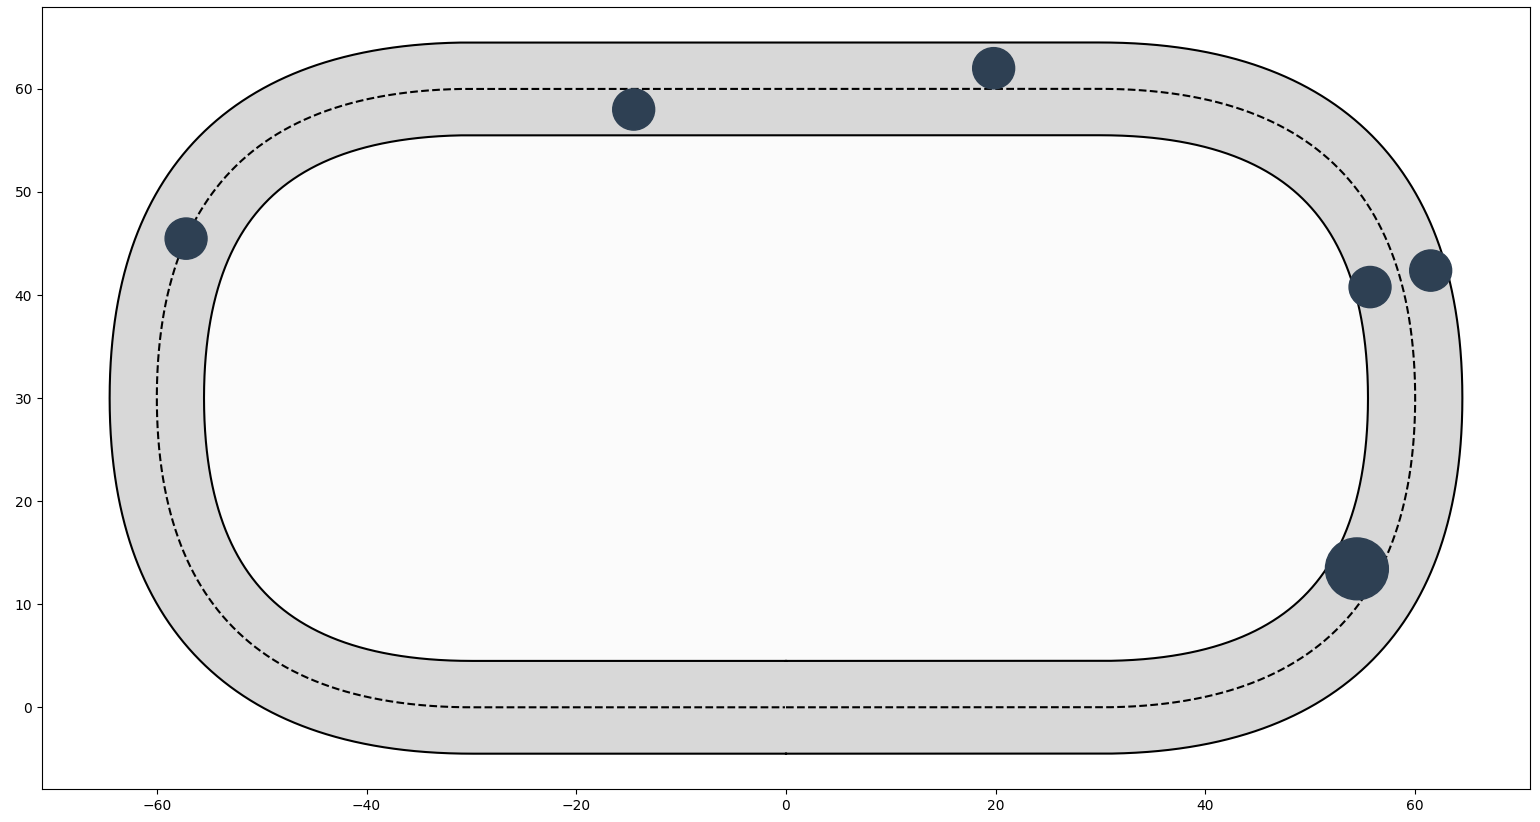
\includegraphics[width=\textwidth]{assets/ippodromo_obstacles.png}
    \caption{Example track with round obstacles}
    \label{ippodromo}
\end{figure} \vspace{0.5cm}
The main features of interest of the track are the following:
\begin{itemize}
    \item centerline position
    \item track curvature
    \item track orientation
\end{itemize}
As for the centerline, we simply evaluate the spline defined through the
waypoints at the curvilinear abscissa $s$. We will define the two spline
functions, one for $x$ and one for $y$ as $x_{spline}(s)$ and $y_{spline}(s)$.\\
The curvature is defined as the inverse of the curvature radius and can be
expressed as
\begin{equation}
    \kappa(s) = \frac{x' \cdot y'' - y' \cdot x''}{\sqrt{(x'^2 + y'^2)^3}}
\end{equation}
where $x'$ and $y'$ are the derivatives of the absolute coordinates with respect
to the curvilinear abscissa $s$. We omitted the dependancy to $s$ in the
righthand-side of the above equation just for notation. The curvature
information is of utmost importance for the controller, since the evolution of
the relative coordinates depends on it. \\
Similarly, the orientation can be expressed as
\begin{equation}
    \phi(s) = \arctan\left(\frac{y'}{x'}\right)
\end{equation}
These two quantities are also needed to convert the relative coordinates to a
global coordinate system. We can express this change of coordinates as such:
\begin{equation}
    \Bigg\{
        \begin{array}{ll}
            x(s,e) =  x_{spline}(s) - sin(\phi(s)) \cdot e\\
            y(s,e) =  y_{spline}(s) + cos(\phi(s)) \cdot e\\
            \varPsi(s,\varPsi) = \phi(s) + \Delta \varPsi
        \end{array}
\end{equation}
This way, it is always possible to identify a pose in the track in global
coordinates, in order to plot the car. More information about the implementation
can be found in
\href{https://github.com/neverorfrog/vehicle-control/blob/main/environment/track.py}{track.py}


\subsection{Discretized model}

An important aspect, which was not mentioned when we treated the models in a
more formal way, is how the models are actually discretized.  What happens is
that, conceptually, the model is still expressed as a symbolic function through
CasADI, as if it were a continuous function. The discretization consists in
adding to the symbolic function an integrator that lets the system transition
from one state by applying a certain input, holding it for a certain amount of
time and integrating the state rate of change, to finally end up into another
state. In the pseudocode, it is line 5 we are talking about. Practically
speaking, what happens is that we create a \textit{discrete ode} in form of a
casadi function by executing the following steps:
\begin{enumerate}
    \item Define the righthand side of the continuous ode as a \textit{symbolic}
    casadi function, namely \[f(state,action,\kappa)\] In our case, taking just
    the singletrack model as an example, the state is the tuple
    \([U_x,U_y,r,\delta,s,e,\Delta\varPsi,t]\) and the action \([F_x,\omega]\).
    Instead, $\kappa$ indicates the curvature of the track. This function
    returns the rate of change of the state. Note that there is the presence of
    both $s$ and $t$, which actually makes no sense conceptually, but the reason
    is that we use the same state for both the $temporalTransition$, depending
    on $dt$ and the $spatialTransition$ depending on $ds$. Simply, in the first
    one $\dot t=1$ and in the second one $s'=1$.
    \item Define the symbolic expression of how the next state would be obtained
    from the current one by applying the rate of change for an interval $h$. For a
    simple Euler integrator, this would correspond to \[state_{n+1}=state_n+h \cdot f(state_n,action_n,\kappa)\]
    \item Embed the symbolic expression into a casadi function which defines the
    discretized dynamics, and as such takes as input the actual state, action
    and curvature tuple, returning the next state: \[state_{n+1}=F(state_n,action_n,\kappa)\]
\end{enumerate}

The implementation of the integrators can be found in
\href{https://github.com/neverorfrog/vehicle-control/blob/main/utils/integrators.py}{integrators.py}
and the dynamical model implementation in
\href{https://github.com/neverorfrog/vehicle-control/blob/main/models/dynamic_car.py}{dynamiccar.py}.
In particular, we decided to use RK4 numerical integrator for the single-track
model because of its accuracy, and the easier Euler method for the pointmass.
For what concerns the discretization of inputs, they are treated in a ZOH
modality, while the path geometry, as said, is discretized through a cubic
spline that can be evaluated through the curvilinear abscissa.




\subsection{MPC Algorithm}
The concepts behind MPC were already addressed in the previous sections; in this
section we will deal with the implementation aspects. As said, most of the
computation happens in the instruction at line 4 of the pseudocode \ref{sim}.
The full implementation of the MPC algorithm can be found in
\href{https://github.com/neverorfrog/vehicle-control/tree/main/controllers/mpc}{cascadedmpc.py}.
We used as linear solver of the optimization problem the solver MA27, which
proved itself faster than the standard solver shipped with CasADI. Regarding the
MPC implementation itself, it can be done in a pretty straightforward way thanks
to the high-level API Opti, which allow to express cost functions and
constraints in a very similar way to the mathematical language.\\
\subsubsection*{Structure of one MPC iteration}
\begin{itemize}
    \item Prepare optimization variables at iteration $n$
    \begin{subequations}
        \begin{eqnarray}
            X_N = [U_{x,k}, U_{y,k}, r_k, \delta_k, s_k, e_k, \Delta \varPsi_k, t_k]_{k=n}^{n+N} \\
            X_M = [V_k, e_k, \Delta \varPsi_k, t_k]_{k=n+N}^{n+N+M} \\
            U_N = [F_{x,k}, \omega_k]_{k=n}^{n+N} \\
            U_M = [F_{x,k}, F_{y,k}]_{k=n+N}^{n+N+M}
        \end{eqnarray}
    \end{subequations}
    \item Initialize parameters $s_0$, $\kappa$, $s$, $ds$ at iteration $n$.
    $s_0$ indicates the current state of the car and it will be the first row of
    the state prediction variables. So we are actually precomputing the
    trajectory of curvilinear abscissae and the spatial step sizes, and also the
    curvatures.
    \item Solve the optimization problem based on the cost function under the
    constraints we talked about before.
    \item Apply the first of the predicted actions, evolve the state of the car and repeat.

\end{itemize}
\subsubsection*{Actual discretization of the NLP}
As said before, inside the prediction horizon, the chosen discretization method
is the one based on spatial discretization. Specifically, the step must be
chosen. For the singletrack, we follow the same approach as in paper, namely
we sample the displacement of the car, considering its speed in real-time,
every $30ms$. This way, we account for big variations of speed during the
entire lap. For the pointmass, instead, we simply choose a static step-size
of $3m$.
\subsubsection*{Horizon Initialization}
Before even starting to solve the optimization problem, we have to properly
initialize it. This is particularly important for computational efficiency.
Here, two things are done:
\begin{itemize}
    \item We initialize the state and action decision variables as the
    predictions from the previous horizon.
    \item We precompute the trajectory of the spatial step sizes, the
    curvilinear abscissae and the curvatures. For the pointmass, it is
    pretty straightforward since the step sizes are predefined. For the
    singletrack, we've used as realtime velocities the predictions of the
    last horizon. After that, we compute the curvatures at the computed
    abscissae. This way, it is not necessary to evaluate the curvature
    spline at every step of the prediction horizon. Indeed, this results in
    a much faster computation.
\end{itemize}
Another thing to mention about the MPC implementation is that we neglected the
terms about the user-defined friction limits depending on road conditions, since
we can't test on a real road. 


\newpage
\section{Experiments}


We've used almost the same data to define the car's model as in \cite{paper}. We
decided to simulate the car as if it were on dry asphalt. Thus, we just changed
the parameters related to the cornering stiffness. Since the authors did the
tests on wet asphalt, and the cornering stiffness is usually higher for dry
asphalts \cite{stiffness}, we decided to raise the cornering stiffness
accordingly. Similarly, the friction values have to take into account that the
asphalt is dry. Letting the car drive on wet asphalt would necessitate extra
parameter tuning and would give additional difficulties that are out of the
scope of this work.
\begin{table}[H]
    \centering
    \caption{Parameters of the dynamic model of the car} \label{params}
    \begin{tabular}{ |c|c|c|c| }
        \hline
        \textbf{Parameter} & \textbf{Symbol} & \textbf{Value} & \textbf{Unit} \\ [0.5ex] 
        \hline
        \hline 
        Vehicle mass & $m$ & 1700 & $kg$\\ 
        \hline
        Inertia & $I_{zz}$ & 3000 & $kg \cdot m^2$\\
        \hline
        Total length & $l$ & 3 & $m$\\
        \hline
        Distance from front axle to CG & $a$ & 1.1 & $m$\\
        \hline
        Distance from rear axle to CG & $b$ & 1.4 & $m$\\
        \hline
        Height of CG & $h_{cg}$ & 0.55 & $m$\\
        \hline
        Modification of tire model & $eps$ & 0.9 & -\\
        \hline
        Maximum engine power & $P_{eng}$ & 170000 & W \\
        \hline
        Drive force distribution & $\chi_{f_d} / \chi_{r_d}$ & 1/0 & -\\
        \hline
        Brake force distribution & $\chi_{f_b} / \chi_{r_b}$ & 0.78 / 0.22 & -\\
        \hline
        Cornering stiffness & $C_{\alpha_f} / C_{\alpha_r}$ & 234000 / 390000 & $N/rad$\\
        \hline
        Steering angle limits & $\delta_{min,max}$ & $\pm$ 0.45 & $rad$ \\
        \hline

    \end{tabular}
\end{table}

\begin{table}[H]
    \centering
    \caption{Parameters of the tire model} \label{env_params}
    \begin{tabular}{ |c|c|c|c| }
        \hline
        \textbf{Parameter} & \textbf{Symbol} & \textbf{Value} & \textbf{Unit} \\ [0.5ex] 
        \hline
        \hline 
        Aerodynamic drag & $C_d$ & 0.4243 & $N/(m/s)^2$ \\
        \hline
        Friction (front/rear wheels) & $\mu_f/\mu_r$ & 0.9 / 0.95 & - \\
        \hline
        Rolling resistance force & $F_{rr}$ & 220 & $N$ \\
        \hline

    \end{tabular}
\end{table}


\begin{table}[H] 
    \centering
    \caption{MPC weights} \label{weights}
    \begin{tabular}{ |c|c|c|c| }
        \hline
        \textbf{Weight} & \textbf{Symbol} & \textbf{Value} & \textbf{Unit} \\ [0.5ex] 
        \hline
        \hline
        Final time & $W_{time}$ & 5 & -\\ 
        \hline
        Terminal speed & $W_{v}$ & 1 & $s/(m/s^2)$\\
        \hline
        Terminal lateral cost & $W_{e_{term}}$ & 1 & $s/m^2$ \\
        \hline
        Terminal course error & $W_{\phi_{term}}$ & 2 & $s/rad^2$ \\
        \hline
        Steering angle & $W_{\dot{\delta}}$ & 4 & $s/(deg/s)^2$ \\
        \hline 
        Input force continuity ($F_x$, $F_y$) & $W_{F}$ & 0.000001 & $s \cdot m / N^2$ \\
        \hline
        Deviation from road descriptor & $W_{rd}$ & 0.001 & $s/m/m^2$ \\
        \hline
        Road Boundary intrusion & $W_{rb}$ & 10 & $s/m/m^2$ \\
        \hline
        Excessive slip angle & $W_\alpha$ & 1500 & s \\
        \hline
        Obstacle avoidance & $W_{obs}$ & 10 & ??? \\
        \hline
        Transition changes & $W_{tr}$ & 0.00001 & $s \cdot m / N^2$ \\
        \hline
    \end{tabular}
\end{table}
Table \ref{weights} shows some typical values of the weights used in the
optimization. These values were chosen through considerations about the model
and also trial-and-error tests. Note that the highest weights are the slip
angle, road boundary and obstacle avoidance. The slip angle is particularly high
because we actually noted that lower values still resulted in the nlp trying to
perform steeper curves, and thus generating high slip angles that would lead to
infeasible lateral forces. 

\subsection{Problem size}
First and foremost, we could compare the dimension of the nlp in terms of
constraints and decision variables. CasADI comes in handy for this task.
Naturally, we expect that the nlp for the cascaded controller is smaller. We
test two configurations: one in singletrack mode with 60 steps, and the other in
cascaded mode with 20 singletrack steps and 35 pointmass steps. \\
\begin{Verbatim}[frame=single,label=Singletrack with 60 steps,labelposition=topline,framesep=10pt]
Number of nonzeros in equality constraint Jacobian...:     3902
Number of nonzeros in inequality constraint Jacobian.:     1380
Number of nonzeros in Lagrangian Hessian.............:     2201

Total number of variables............................:      600
Total number of equality constraints.................:      480
Total number of inequality constraints...............:      480

Number of objective function evaluations             = 18
Total seconds in IPOPT                               = 0.114 ms
\end{Verbatim} 
\vspace{1mm}
\begin{Verbatim}[frame=single,label=Cascaded with 20+35 steps,labelposition=topline,framesep=10pt]
Number of nonzeros in equality constraint Jacobian...:     1989
Number of nonzeros in inequality constraint Jacobian.:      565
Number of nonzeros in Lagrangian Hessian.............:     1275

Total number of variables............................:      550
Total number of equality constraints.................:      335
Total number of inequality constraints...............:      230

Number of objective function evaluations             = 22
Total seconds in IPOPT                               = 0.050 ms
\end{Verbatim}
Even though the number of total steps is almost the same, the singletrack
configuration has clearly more variables and constraints. Moreover, we should
consider that in the MPC all the variables are inside a single CasADI matrix
(whose size if fixed apriori) and that the pointmass has less state variables
than the singletrack model. Hence, the number of "active variables" is even less
than the number shown above. In fact, a better indicator is the number of
constraints, especially the inequalities, and the jacobian and hessian
dimension. The latter is almost halved for the cascaded configuration. This is
due to the fact that the pointmass model neglects the terms concerning steering,
namely the minimization of steering velocities and slip angle cost term. The
neglected constraints are the ones concerning the tire model and, again, the
steering inputs. For what concerns the effective duration of the MPC iteration,
the cascaded controller takes signifantly less time, despite needing more
evaluations. Also, despite the number of steps being almost the same, fewer
pointmass steps are necessary, because the spatial step size can be chosoen
bigger thatn with the singletrack. That caused by the fact that the pointmass is
non subject to the delicate yaw dynamics. Anyway, just to visualize and be aware
of how much the pointmass model impacts the horizon, the two horizon lengths are
shown in figure \ref{horizons}.

\subsection{Cascaded vs Singletrack on a simple track}

The first set of tests was carried out on a pretty simple track, as the one in Figure
\ref{ippodromo}, without obstacles for the moment. We compare different configurations
for both singletrack and cascaded models, changing the length of the horizon and the 
maximum speed velocity. We report the results below. We tried also other configurations,
but the ones reported here are the most interesting ones. The
first column indicates the number of iterations per lap and the second the lap
time. The third column indicates the average time per iteration of the MPC,
while the fourth and fifth column represent the average speed and the average
force input.

\begin{table}[h] 
    \centering
    \caption{Performance of various controller configurations} \label{simulations}
    \begin{tabular}{|c||c|c|c|c|c|}
        \hline
        \textbf{Controller} & \textbf{Iter.} & \textbf{Lap} & \textbf{Time} & \textbf{Av.$U_x$} & \textbf{Av.|$F_x$|} \\ [0.5ex] 
        \hline
        \hline
        Singletrack $N=50$, $V_{max}=18m/s$ & 442 & $22.05 s$ & $93 ms$ & $14.26 m/s$ & $2661.67 N$\\
        \hline
        Singletrack $N=50$, $V_{max}=20m/s$ & 448 & $22.35 s$ & $105 ms$ & $14.07 m/s$ & $3273.58 N$\\
        \hline
        Singletrack $N=60$, $V_{max}=18m/s$ & 433 & $21.60 s$ & $81 ms$ & $14.44 m/s$ & $2375.56 N$\\
        \hline
        Singletrack $N=60$, $V_{max}=20m/s$ & 428 & $21.35 s$ & $127 ms$ & $14.58 m/s$ & $2543.66 N$\\
        \hline
        Cascaded $N=20, M=15, V_{max}=18m/s$ & 432 & $21.55 s$ & $42 ms$ & $14.41 m/s$ & $2083.51 N$\\
        \hline
        Cascaded $N=20, M=25, V_{max}=18m/s$ & 424 & $21.15 s$ & $47 ms$ & $14.64 m/s$ & $2337.79 N$\\
        \hline
        Cascaded $N=20, M=35, V_{max}=18m/s$ & 418 & $20.85 s$ & $47 ms$ & $14.75 m/s$ & $2588.77 N$\\
        \hline
        Cascaded $N=20, M=35, V_{max}=20m/s$ & 418 & $20.85 s$ & $63 ms$ & $14.77 m/s$ & $2591.64 N$\\
        \hline
    \end{tabular}
\end{table}

\begin{figure}[H] 
    \centering
        \begin{subfigure}{0.9\textwidth} 
        \centering
        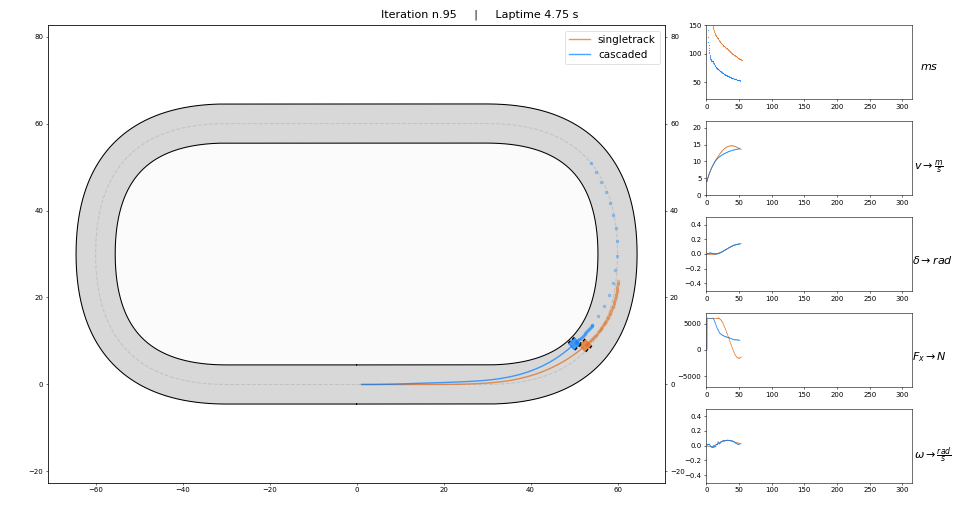
\includegraphics[width=\textwidth]{assets/horizon_shorter.png}
        \subcaption{Cascaded with $N=20, M=15$}
    \end{subfigure}
    \begin{subfigure}{0.9\textwidth}
        \centering
        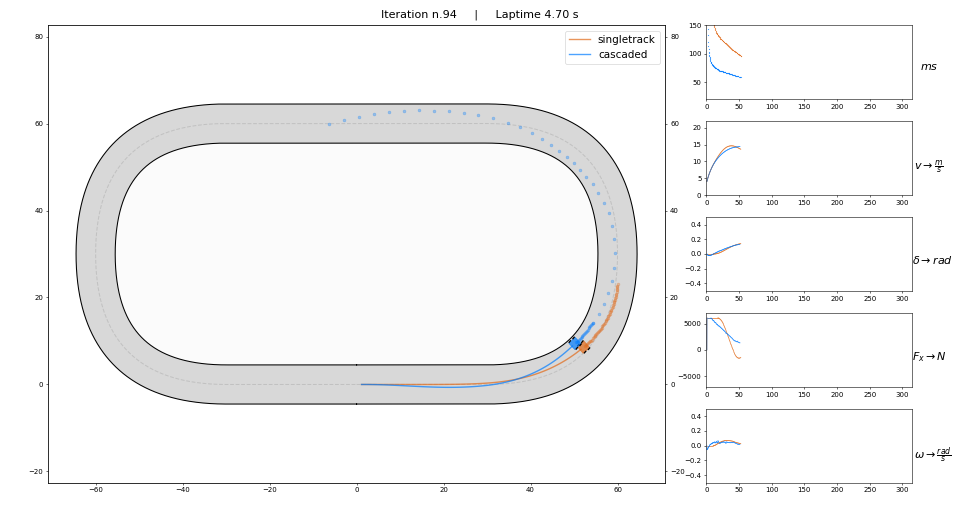
\includegraphics[width=\textwidth]{assets/horizon_longer.png}
        \subcaption{Cascaded with $N=20, M=35$}
    \end{subfigure}
    \caption[short]{Comparison of two horizon lengths against the singletrack}
    \label{horizons}
\end{figure}

\paragraph{Computational efficiency}
The cascaded controller halves the average computation time with respect to the
singletrack. That alone demonstrates the effectiveness of using such a
controller as opposed to using the singletrack model for the whole prediction
horizon. Considering that the sample time is $50ms$ in our experiments, the
computation time of the singletrack controller exceeds by fare realtime
requirements. Moreover, in the first iterations, the singletrack reaches $130ms$
per iterations, which is absolutely prohibitive. Of course, when adding more
pointmass steps, the time per iteration increases, but not significantly. In
fact, when passing from $M=25$ to $M=35$, the increase in computation time is
negligible.

\paragraph{Laptime}
Considering just the first two rows, the laptime is almost the same, but there's
a big caveat to that. The singletrack controller actually exceeds the slip angle
limits at the third curve by $0.16 deg$, generating infeasible lateral forces.
This is not surprising, since the segment before is straight and long enough to
reach a relatively high speed, while the prediction horizon is not far-sighted
enough to see how much curvature the track has. Thus, it tries to recover the
track path by braking and steering as much as it can. Moreover, if we increase
the maximum speed of the controllers to $20 m/s$ and keep every other weight
exactly the same as before, the singletrack actually goes outside as in figure
\ref{singletrack_outside}, while the cascaded' performance is enhanced. We also
tried increasing the maximum speed even more, with the singletrack going
completely out of the track and the cascaded always performing well. That is
simply thanks to the longer horizon. Of course, one could argue that the weight
on the laptime should be decreased in order regain a safer driving profile. On
the other hand, this would probably result in a 

\paragraph{Driving profile}
It is interesting to notice that with a longer prediction horizon, the driving
profile changes and assumes a more aggressive behavior. Specifically, before the
first curve, which is to the left, there is an inflection to the right. This is
typical of racing cars: the goal is to break anticipately and take the curve
from a more external point, in order to hit the so-called "apex", namely the
nearest point to the internal border of the curve, at the highest possible
speed. Another consequence, as we can observe from figure \ref{race_ippodromo},
is that the flex is hit slightly later with the longer horizon. Before the third
curve the behavior is similar: the car keeps going on the external side of the
track for a longer time, in order to take the turn with higher speed. An
indicator of this more aggressive driving behavior is the mean squared (lateral)
error. As expected, the singletrack controller is more conservative in that
sense; it tries to stay as much as possible at the center of the track.
Meanwhile, the cascaded controller roams the track while also allowing itself to
drive near the border in order to reduce laptime.
\begin{table}[H]
    \centering
    \caption{Analysis of mean squared error and laptime}
    \begin{tabular}{|c||c|c|c|}
        \hline
        \textbf{Controller} & \textbf{Iter.} & \textbf{Lap} & \textbf{MSE} \\ [0.5ex] 
        \hline
        \hline
        Singletrack $N=60$ & 432 & $21.60 s$ & $1.55 m$ \\
        \hline
        Cascaded $N=20, M=15$ & 430 & $21.50 s$ & $3.37 m$ \\
        \hline
        Cascaded $N=20, M=35$ & 417 & $20.85 s$ & $3.20 m$ \\
        \hline
    \end{tabular}
\end{table}
\begin{figure}[H]
    \centering
    \begin{subfigure}{0.9\textwidth}
        \centering
        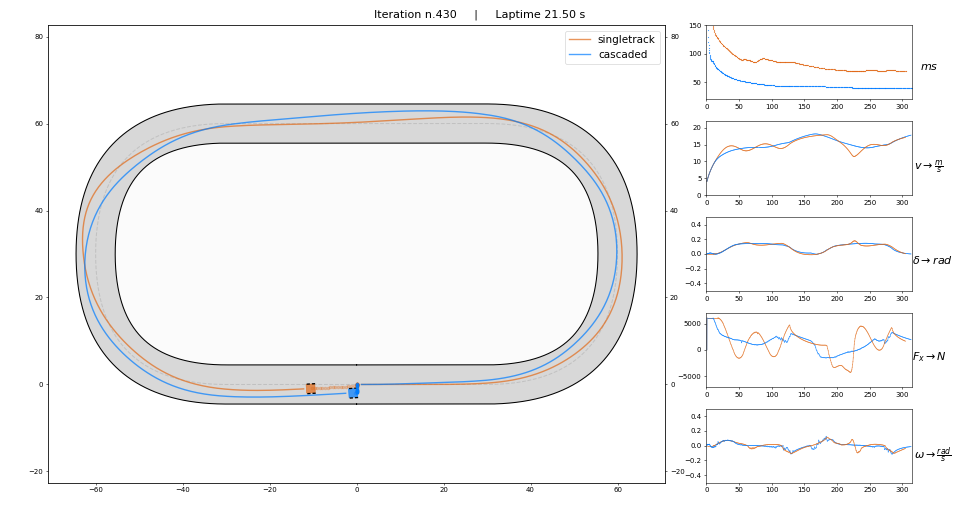
\includegraphics[width=\textwidth]{assets/race1_ippodromo.png}
        \subcaption{Maximum speed of $18 m/s$}
    \end{subfigure}
    \begin{subfigure}{0.9\textwidth}
        \centering
        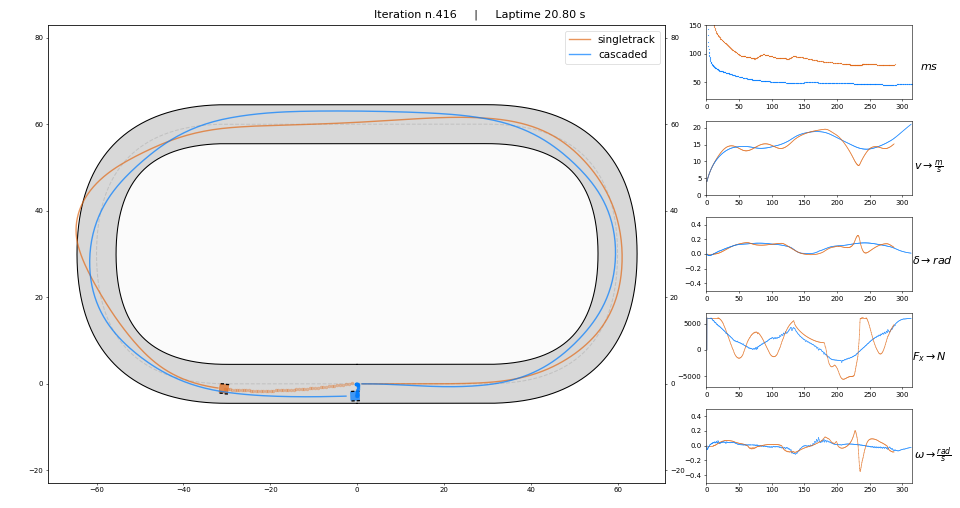
\includegraphics[width=\textwidth]{assets/race3_ippodromo.png}
        \subcaption{Maximum speed of $20 m/s$}
        \label{singletrack_outside}
    \end{subfigure}
    \caption[short]{Comparison of two cascaded controllers}
    \label{race_ippodromo}
\end{figure}
\paragraph{$F_x$ usage}
The average force usage cannot be analysed separately from the other parameters
of table \ref{simulations}. So, let's start with the first two rows of the
table, and then we will extend the considerations to the other ones. The
single-track model is the one that takes the longest time to finish the circuit,
even if it has a (slightly) higher average speed (but almost the same) and
higher average force. That may seem counterintuitive, since with higher force,
there should be higher speed. Actyally, the cascaded model can optimize in a
better way its velocity and the distribution of the force along the track, due
to its long horizon planning capacity. More intuitively, the braking happens in
anticipation, rather than after noticing the curve is too steep. Hence, the
average speed is almost the same, although the force usage is higher.
Considering now the third and fourth row of the table, we notice that the
increase in force usage and average speed are proportional to each other,
resulting in the last cascaded model having a considerably higher average speed
(considering how short the track is) than the singletrack. This overview
suggests how this cascaded model is the best one between the three considered,
because it can balance the usage of the force in order to reach better
performances.\\
As an extreme case, the last row of table \ref{simulations} shows a singletrack
controller with 60 steps and a higher maximal allowed speed. The simulation of
this controller is shown in figure \ref{singletrack_outside}. As already pointed
out, previously, the car goes outside the track at a certain point. Indeed, the
average speed decreases while the force usage increases by far, due to the
excessive braking to recover the track path.

\paragraph{Pushing the car to its physical boundaries}
An important idea, for which this work shall serve as proof-of-concept, is to
test how the car handles being pushed to its physical boundaries. Such
considerations can be made by exploiting "almost infeasible" situations in the
optimization. In particular, we can consider how sensitive the MPC control
algorithm can be, depending on its weights.  
\begin{figure}[H]
    \centering
    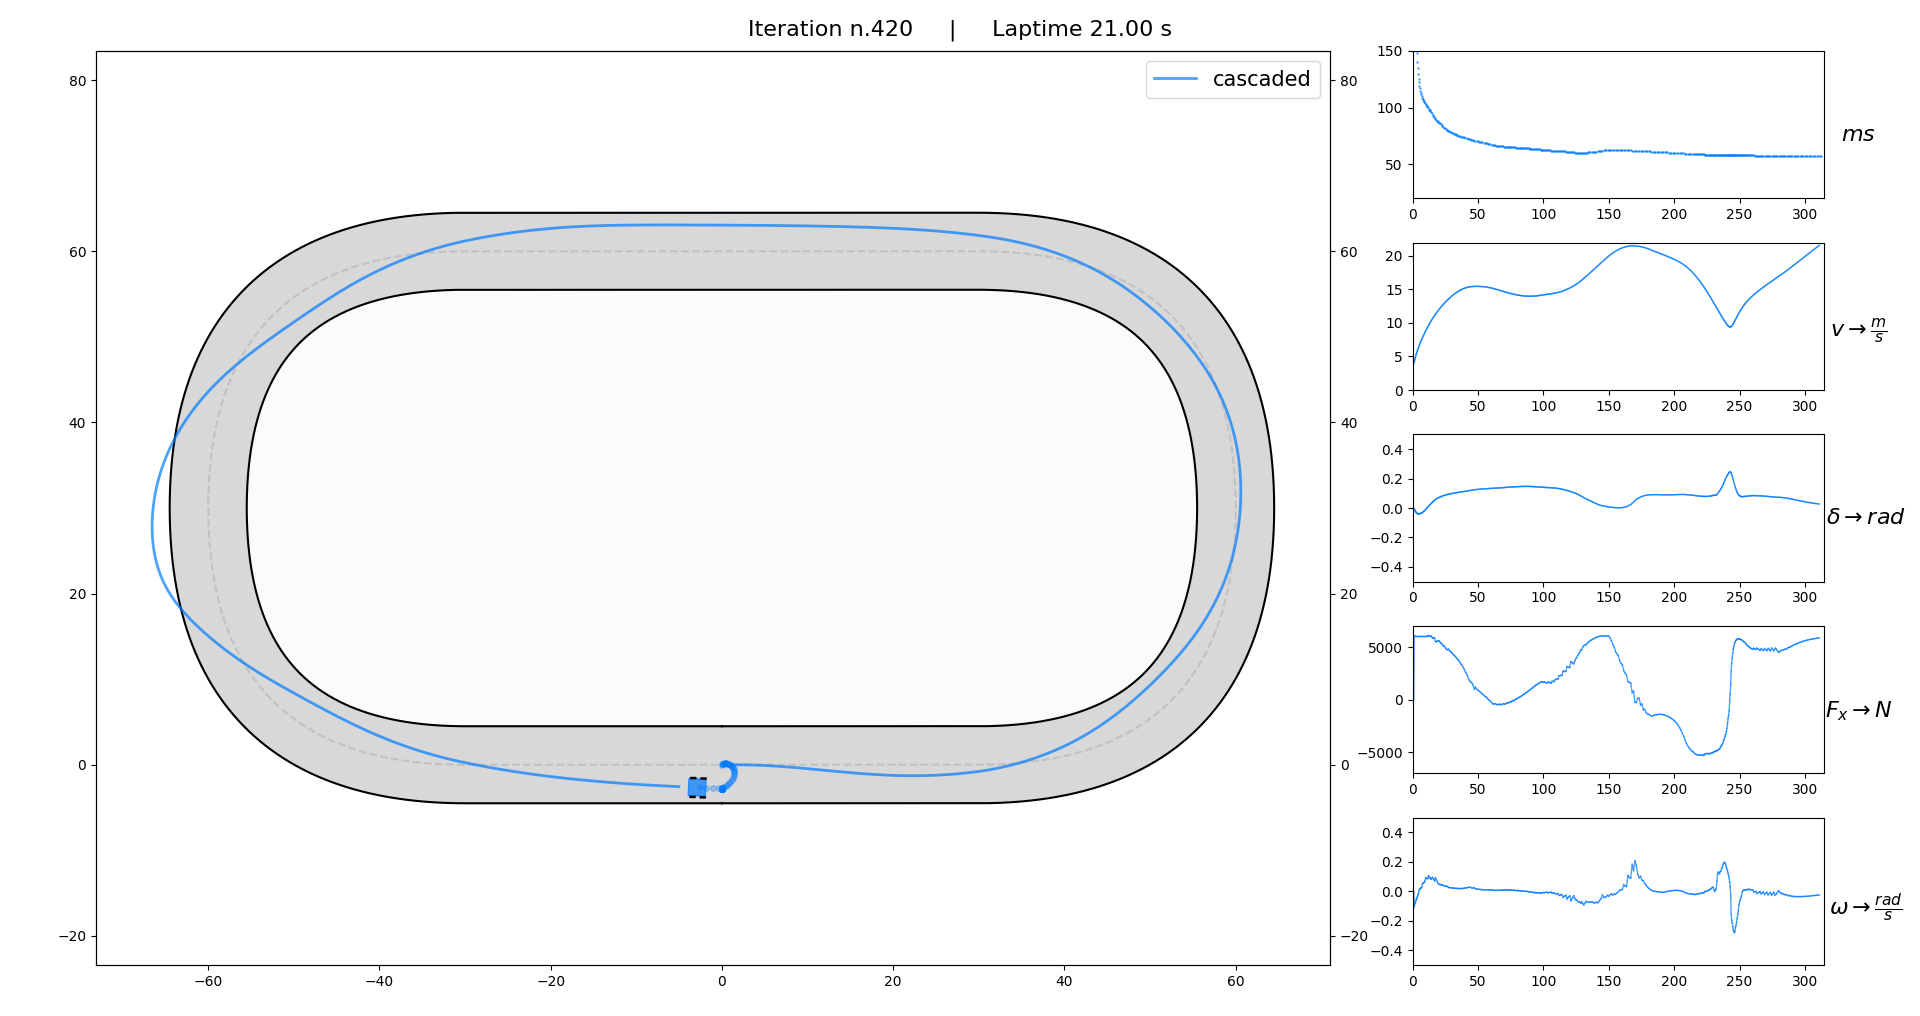
\includegraphics[width=0.8\textwidth]{assets/cascaded_high_laptime_weight.png}
    \caption{$W_{t}$ = 50}
    \label{hightime}
\end{figure}
We have already seen that the singletrack controller is keen on exceeding the
slip angle limits, due to having a shorter horizon. This condition can also
happen if, for example, we increase the weight on the laptime. Intuitively, the
higher the laptime weight, the more the car will try to reduce the laptime. Just
as an illustrative example, if we increase the laptime weight (with respect to
\ref{weights}) to $50$, the result is the one in figure \ref{hightime}, that is,
the car goes outside the track. That is just to say, that handling a dynamic
model at its physical limits can be difficult in terms of tuning MPC weights.

\subsection{Adding obstacles to the track}

We also experimented adding obstacles to the track and comparing the performance
depending on the weight in the cost function. The controller parameters are the
same, just with the added cost weight. Incidentally, the singletrack controller
was not even able to finish the track without going into a numerical
infeasibility situation. 
\begin{figure}[H]
    \centering
    \begin{subfigure}{0.9\textwidth}
        \centering
        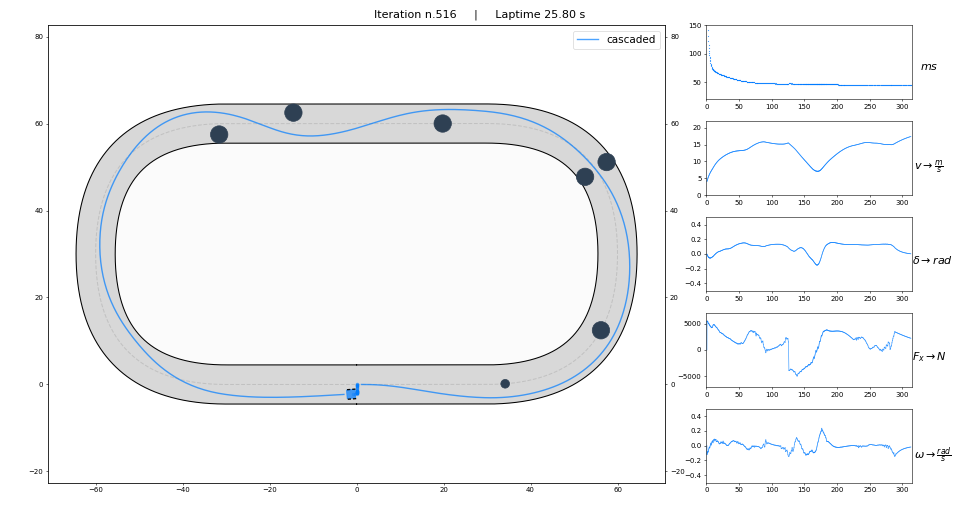
\includegraphics[width=\textwidth]{assets/obstacles1_ippodromo.png}
        \subcaption{$W_{obs}$ = 10}
        \label{obs1}
    \end{subfigure}
    \begin{subfigure}{0.9\textwidth}
        \centering
        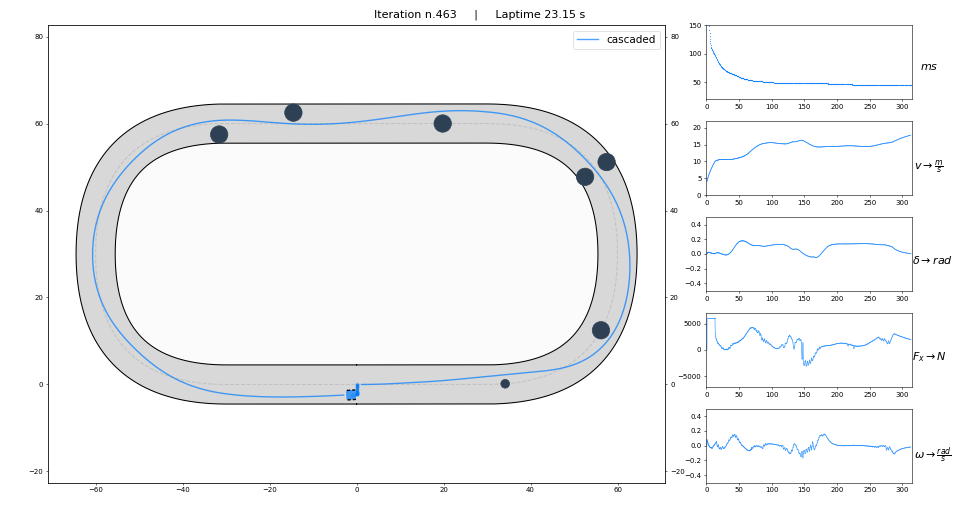
\includegraphics[width=\textwidth]{assets/obstacle2_ippodromo.png}
        \subcaption{$W_{obs}$ = 1}
    \end{subfigure}
    \caption[short]{Comparison of two cascaded controllers with obstacles}
\end{figure}
\begin{table}[H] 
    \centering
    \caption{Different cascaded controllers ($N=20$, $M=15$) depending on $W_{obs}$} \label{obstacles_ippodromo}
    \begin{tabular}{|c||c|c|c|c|c|}
        \hline
        \textbf{Controller} & \textbf{Iter.} & \textbf{Lap} & \textbf{Time} & \textbf{Av.Speed} & \textbf{Av.$F_x$} \\ [0.5ex] 
        \hline
        \hline
        $W_{obs}$ = 10 & 518 & $25.85 s$ & $44 ms$ & $12.43 m/s$ & $2473.79 N$\\
        \hline
        $W_{obs}$ = 1 & 465 & $23.20 s$ & $44 ms$ & $13.64 m/s$ & $1903.64 N$\\
        \hline
    \end{tabular}
\end{table}
As pretty much expected, the controller with a lower weight on obstacle
avoidance is more aggressive, going very near the obstacles. This results in a
higher average speed, thus a lower laptime. It also results in a lower average
force usage, due to the reduced braking.
\begin{figure}[H]
    \centering
    \begin{subfigure}{0.9\textwidth}
        \centering
        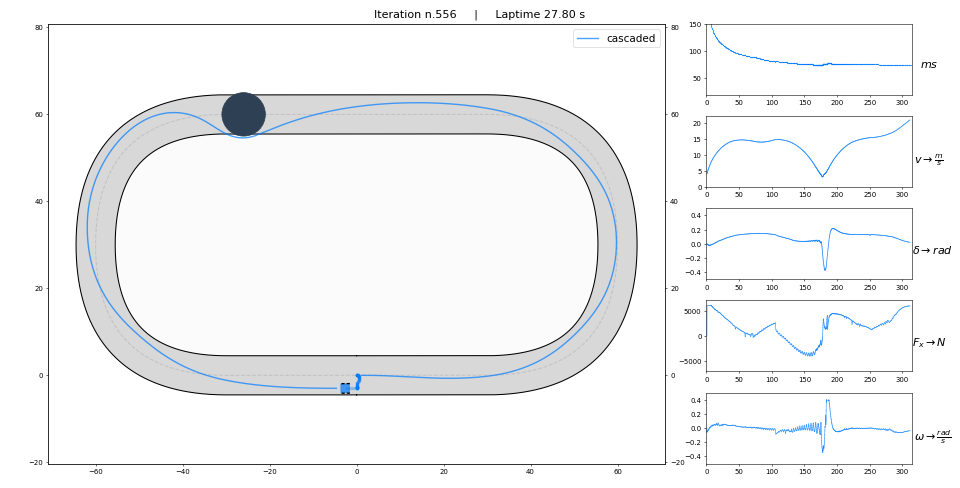
\includegraphics[width=\textwidth]{assets/giant2.png}
        \subcaption{$W_{obs}$ = 10}
        \label{giant2}
    \end{subfigure}
    \begin{subfigure}{0.9\textwidth}
        \centering
        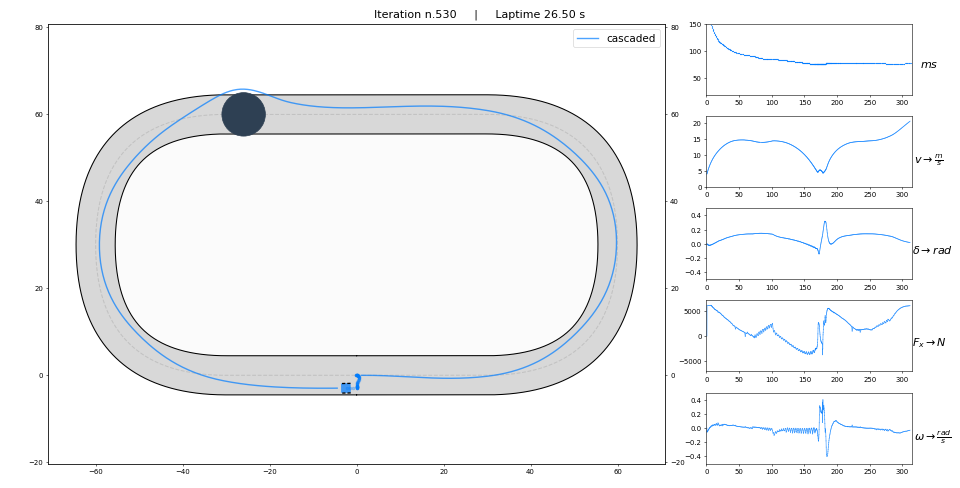
\includegraphics[width=\textwidth]{assets/giant1.png}
        \subcaption{$W_{obs}$ = 50}
        \label{giant1}
    \end{subfigure}
    \caption[short]{Comparison of two cascaded controllers with giant obstacle}
\end{figure}
We tried also another experiment, where one obstacle covers the entire width of the 
track. This is an important test that allows to verify if the model is quite robust,
because of how we modeled the optimization problem. How explained in \ref{cost_section},
both terms about the road boundary intrusion and obstacle avoidance are modeled
as terms in the cost function instead of as constraints. This choice allows to make the
problem feasible also in cases like this. As shown in the figures \ref{giant1} and 
\ref{giant2}, the car assumes exactly the behavior we would like it to have, that is, 
it goes slightly outside the track to avoid the obstacle, and then it comes back into 
the boundaries. 
The difference between these two examples is in the values of the weights 
about the obstacle avoidance. In particular, in the former we considered a weight $W_{obs}=10$ 
(the same situation shown in the example \ref{obs1}), while in the latter the weight is
$W_{obs}=50$. We can notice like the first one is almost an impossible case in the reality,
due to the high proximity of the car to the surface of the object. On the opposite, the
second configuration handles these type of situations better.

\subsection{Longer track with steeper curves}

We experimented also on a different and longer (more realistically) track that
has also steeper curves.

\begin{figure}[H]
    \centering
    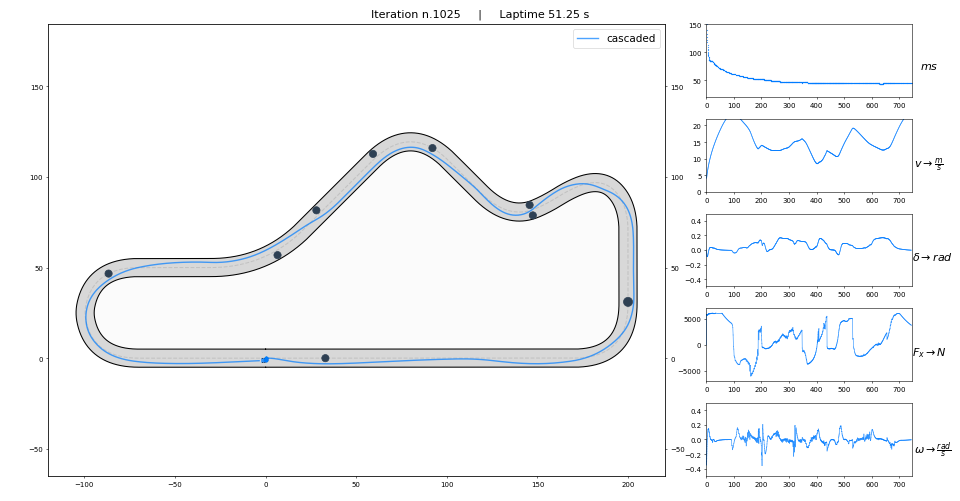
\includegraphics[width=0.95\textwidth]{assets/obstacles_shoe.png}
    \label{shoe}
    \caption{Cascaded controller on longer track with obstacles}
\end{figure}
The laptime difference is even more exaggerated, more than 1 second. Also, it is
interesting to notice that the computational efficiency is pretty much the same
for the cascaded controller (under 50 ms), while for the singletrack it is even
worse than before. In particular, in figure \ref{singletrack_shoe}, we can
observe a spike in the computational time, corresponding to the first (the
steepest one) curve. Since the car has to recover the track without crossing the
boundaries, the optimizer takes much more to find a solution. Moreover, again,
the generated forces by the singletrack are infeasible in practice, since it
tries to brake too much while steering, impressing too much lateral force. These
issues don't presente themselves in the cascaded controller. 
\begin{figure}[H]
    \centering
    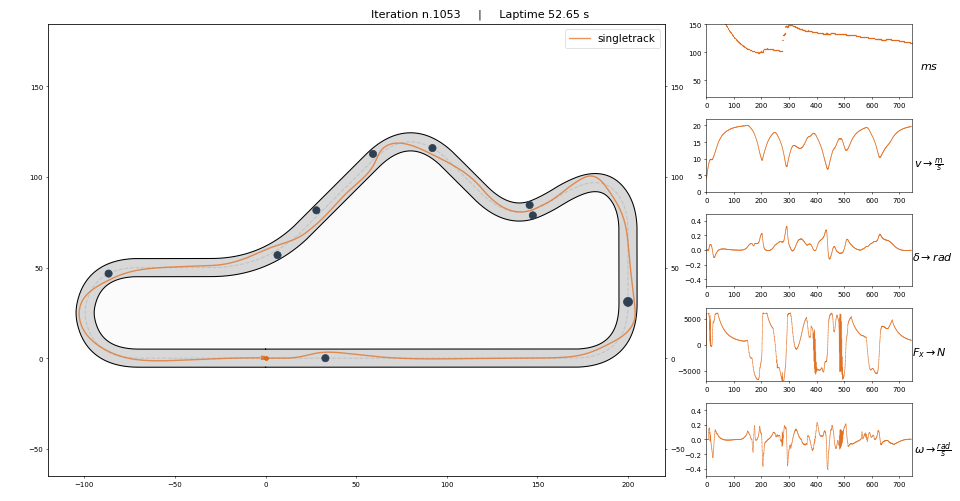
\includegraphics[width=0.95\textwidth]{assets/singletrack_obstacles_shoe.png}
    \label{singletrack_shoe}
    \caption{Singletrack controller on longer track with obstacles}
\end{figure}


\subsection{Kinematic Model}

The singularity limitation of the dynamic model can be addressed by using a
kinematic model instead. The structure of the NLP is pretty much the same. Of
course, the computation times are much reduced, namely from $50ms$ to $20ms$.
Ideally, the kinematic model should be used at low speeds. After reaching a
sufficient speed, we could switch to the dynamic model.
\begin{figure}[H]
    \centering
    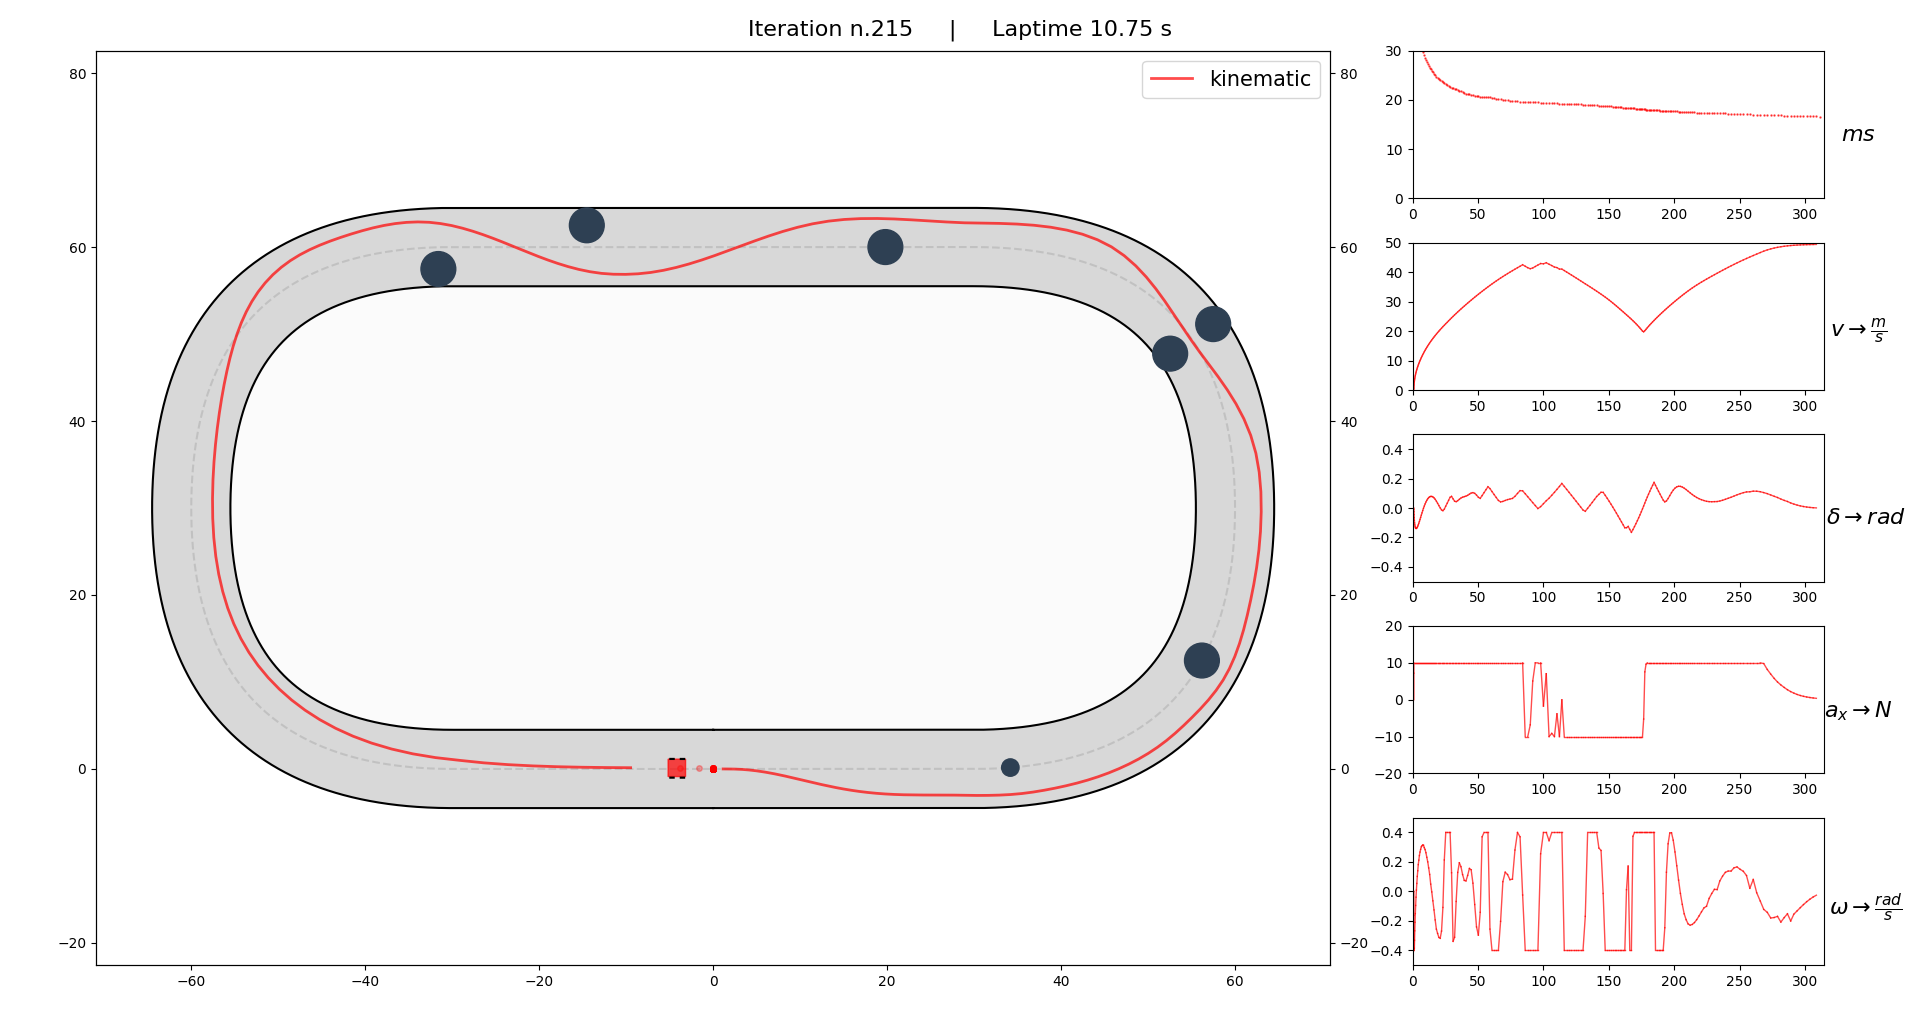
\includegraphics[width=0.95\textwidth]{assets/kinematic_ippodromo.png}
    \label{kin}
    \caption{Kinematic controller}
\end{figure}




\newpage
\section{Conclusion}

In this work we proposed the implementation and experimentation of the cascaded
MPC algorithm. We showed through the experiments that the algorithm effectively
works and the premises are right. Of course, there are still some limitations to
this approach. One could be that the manual tuning of the MPC weights is not
easy. It requires domain expertise about the dynamical model and the task at
hand. Thus, a possible extension to this work could be to use a learning
approach that lifts the programmer from hardcoding the model and the weights.
This could be done maybe with an iterative learning approach and where both
models, the singletrack and the pointmass can be predicted by two neural networks.

\bibliographystyle{unsrt}
\bibliography{references}

\end{document}
